\providecommand{\topdir}{../..} 
\documentclass[\topdir/lecture\_notes.tex]{subfiles}
\graphicspath{{\subfix{./images/}}}

\begin{document}

\section{An Informal Introduction to Stochastic Calculus}
Brownian motion is a continuous-time scalar stochastic process such that, given the initial value $x_{0}$ at time $t=0$, the random variable $x_{t}$ for any $t>0$ is normally distributed with mean $x_{0}+\mu_t$ and variance $\sigma^{2}_t$. The parameter $\mu$ measures the trend, and $\sigma$ the volatility, of the process. This process was first formulated to represent the motion of small particles suspended in a liquid. We shall sometimes refer to a ``particle'' performing the Brownian motion, $x_{t}$ as its ``position'', and a graph of $x_{t}$ against $t$ as its ``path''.

We can think of Brownian motion as the cumulation of independent identically distributed normal increments, the infinitesimal random increment $dx$ over the infinitesimal time $dt$ having mean $\mu dt$ and variance $\sigma^{2} dt$. Just as we would write a general normal $(\mu, \sigma)$ variable as $\mu+\sigma w$ where $w$ is a standard normal random variable of zero mean and unit variance, we can write
\begin{align}
dx=\mu dt+\sigma dw \label{eq:brownian_motion}
\end{align}
where $w$ is a standardized Brownian motion (Wiener process) whose increment $dw$ has zero mean and variance $dt$. This is the usual shorthand notation for Brownian motion. Figure \ref{fig:bm_paths_normal} gives a visual summary of the last two paragraphs.
\begin{figure}
    \centering
    \begin{tikzpicture}[ % Define Normal Probability Function
declare function={
            normal(\x,\m,\s) = 1/(2*\s*sqrt(pi))*exp(-(\x-\m)^2/(2*\s^2));
        },
    declare function={invgauss(\a,\b) = sqrt(-2*ln(\a))*cos(deg(2*pi*\b));}
       ]
\begin{groupplot}[group style={group size=2 by 3},height=6cm,width=6cm,
    %no markers,
    domain=0:12,
    zmin=0, zmax=1,
    xmin=0, xmax=3,
    samples=200,
    samples y=0,
    view={40}{30},
    axis lines=middle,
    enlarge y limits=false,
    xtick={0.5,1.5,2.5},
    xmajorgrids,
    xticklabels={},
    ytick=\empty,
    xticklabels={$t_1$, $t_2$, $t_3$},
    ztick=\empty,
    xlabel=$t$, xlabel style={at={(rel axis cs:1,0,0)}, anchor=west},
    ylabel=$x$, ylabel style={at={(rel axis cs:0,1,0)}, anchor=south west},
    zlabel=Probability density, zlabel style={at={(rel axis cs:0,0,0.5)}, rotate=90, anchor=south},
    set layers
  ]
\pgfplotsinvokeforeach{0.5,0.9,1.3,1.7,2.1,2.5}
{\nextgroupplot[]
  \addplot3 [samples=2, samples y=0, domain=0:3] (x, {1.5*(x-0.5)+3}, 0);

  \addplot3 [draw=none, fill=black, opacity=0.25, only marks, mark=dot, mark
  layer=like plot, samples=30, domain=0.1:2.9, on layer=axis background,overlay]
  (#1, {1.5*(#1-0.5)+3+invgauss(rnd,rnd)*#1}, 0);

  \begin{pgfonlayer}{axis background}
  \begin{scope}
  \clip (0,0,0) -- (#1,0,0)  -- (#1,12,0) -- (0,12,0) -- cycle;
  \draw[red,no marks,name path=rp1] plot coordinates {\mytabone};
  \draw[red,no marks,name path=rp2] plot coordinates {\mytabtwo};
  \draw[red,no marks,name path=rp3] plot coordinates {\mytabthree};
  \draw[red,no marks,name path=rp4] plot coordinates {\mytabfour};
  \end{scope}
  \draw [gray, on layer=axis background] (#1, 2.25+1.5*#1, 0) -- 
  (#1, 2.25+1.5*#1, {normal(0,0,0.5*#1+0.25)});
  \draw [gray, on layer=axis background,name path=vert] (#1,0,0) -- (#1,12,0);
  \end{pgfonlayer}
  \path[name intersections={of=vert and rp1,by={x1}},
  name intersections={of=vert and rp2,by={x2}},
  name intersections={of=vert and rp3,by={x3}},
  name intersections={of=vert and rp4,by={x4}}];
  \draw [fill=red, opacity=0.75, only marks, mark=dot] plot coordinates 
  {(x1) (x2) (x3) (x4)};
  \addplot3 [blue, very thick] (#1, x, {normal(x, 2.25+1.5*#1,0.5*#1+0.25)});
  }
\end{groupplot}
\end{tikzpicture}
\caption{Paths of Brownian motion $x_t$ are plotted in red. The different panels show the evolution of paths and of the normal distribution of $x_t$ in blue as time goes by. The mean of the distribution is on black straight line. The variance of the distribution increases with $t$.}\label{fig:bm_paths_normal}
\end{figure}

\subsection{Random Walk Representation}
We approximate Brownian motion by a discrete random walk. Then the normal distribution arises as the limit of a sum
of independent binary variables $\Delta x$ over discrete time intervals $\Delta t$, when these go to zero in a particular way.

Divide time into discrete periods of length $\Delta t$, and let space consist of discrete points along a line, $\Delta h$ being the step-length or the distance between successive points. Let $\Delta x$ be a random variable that follows a random walk: in one time period it moves up one step in space with probability $p$, and one step down with probability $q=1-p$. Note: $\Delta h$ is a given positive number, and $\Delta x$ is a random variable that takes values $\pm \Delta h$. Figure \ref{fig:random_walk} shows all this compactly. We see various possible paths, with time marching downward and position shown horizontally. At each point in time and space, the probability of reaching it is also shown.

The mean of $\Delta x$ is
\begin{align}
    E[\Delta x]=p \Delta h+q(-\Delta h)=(p-q) \Delta h.
\end{align}
Also,
\begin{align*}
    E\left[(\Delta x)^{2}\right]=p(\Delta h)^{2}+q(-\Delta h)^{2}=(\Delta h)^{2},
\end{align*}
so the variance of $\Delta x$ is
\begin{align}
    \operatorname{Var}[\Delta x] & =E\left[(\Delta x)^{2}\right]-(E[\Delta x])^{2} \\
    & =\left[1-(p-q)^{2}\right](\Delta h)^{2}=4 p q(\Delta h)^{2}
\end{align}

\begin{figure}
    \centering
    \begin{tikzpicture}[scale=0.8]
	\tikzstyle{every label}=[fill=white]
	\begin{pgfonlayer}{nodelayer}
		\node [shape=circle, fill=black, inner sep=0.5mm, draw, label={above:$x_0$}] (0) at (0, 0) {};
		\node [style=none, label={above left:$q$}] (1) at (-2, -2) {};
		\node [style=none, label={above left:$q^2$}] (2) at (-4, -4) {};
		\node [style=none, label={above left:$q^3$}] (3) at (-6, -6) {};
		\node [style=none, label={above right:$p$}] (4) at (2, -2) {};
		\node [style=none, label={above right:$p^2$}] (5) at (4, -4) {};
		\node [style=none, label={above right:$p^3$}] (6) at (6, -6) {};
		\node [style=none, label={[shift={(0.4,0)}]right:$2pq$}] (7) at (0, -4) {};
		\node [style=none, label={[shift={(0.4,0)}]right:$3pq^2$}] (8) at (-2, -6) {};
		\node [style=none, label={[shift={(0.4,0)}]right:$3p^2q$}] (9) at (2, -6) {};
		\node [style=none] (10) at (-7, -7) {};
		\node [style=none] (11) at (-5, -7) {};
		\node [style=none] (12) at (-3, -7) {};
		\node [style=none] (13) at (-1, -7) {};
		\node [style=none] (14) at (1, -7) {};
		\node [style=none] (15) at (3, -7) {};
		\node [style=none] (16) at (5, -7) {};
		\node [style=none] (17) at (7, -7) {};
	\end{pgfonlayer}
	\begin{pgfonlayer}{edgelayer}
		\draw [style=arrow] (0.center) to (1.center);
		\draw [style=arrow] (1.center) to (2.center);
		\draw [style=arrow, in=45, out=-135] (2.center) to (3.center);
		\draw [style=arrow] (0.center) to (4.center);
		\draw [style=arrow] (4.center) to (5.center);
		\draw [style=arrow] (5.center) to (6.center);
		\draw [style=arrow] (4.center) to (7.center);
		\draw [style=arrow] (1.center) to (7.center);
		\draw [style=arrow] (7.center) to (8.center);
		\draw [style=arrow] (7.center) to (9.center);
		\draw [style=arrow] (5.center) to (9.center);
		\draw [style=arrow] (2.center) to (8.center);
		\draw [style=dash arrow] (3.center) to (10.center);
		\draw [style=dash arrow] (3.center) to (11.center);
		\draw [style=dash arrow] (8.center) to (12.center);
		\draw [style=dash arrow] (8.center) to (13.center);
		\draw [style=dash arrow] (9.center) to (14.center);
		\draw [style=dash arrow] (9.center) to (15.center);
		\draw [style=dash arrow] (6.center) to (16.center);
		\draw [style=dash arrow] (6.center) to (17.center);
	\end{pgfonlayer}
	\draw [style=reversearrow] (-9,0) to (-9,-1) node[label=left:{$\Delta t$}] {};
	\draw [style=arrow] (-9,-1) to (-9,-2) ;
	\draw [style=reversearrow] (-8,0.8) to (-7,0.8)  node[label=above:{$\Delta h$}] {};
        \draw [style=arrow] (-7,0.8) to (-6,0.8) {};
		
	\draw[xstep=2,ystep=2] (-8,0) grid (8,0);
	\draw[xstep=2,ystep=2] (-8,-2) grid (-2,-2);
	\draw[xstep=2,ystep=2] (-8,-4) grid (-4,-4);
	\draw[xstep=2,ystep=2] (-8,-6) grid (-6,-6);
	
	\draw[xstep=2,ystep=2] (-8,0) grid (-8,-8);
	\draw[xstep=2,ystep=2] (-6,0) grid (-6,-6);
	\draw[xstep=2,ystep=2] (-4,0) grid (-4,-4);
	\draw[xstep=2,ystep=2] (-2,0) grid (-2,-2);
	
	\draw[xstep=2,ystep=2] (8,0) grid (8,-8);
	\draw[xstep=2,ystep=2] (6,0) grid (6,-6);
	\draw[xstep=2,ystep=2] (4,0) grid (4,-4);
	\draw[xstep=2,ystep=2] (2,0) grid (2,-2);
    \end{tikzpicture}
    \caption{Random walk representation.}\label{fig:random_walk}
\end{figure}

A time interval of length $t$ has $n=t / \Delta t$ such discrete steps. Since the successive steps of the random walk are independent, the cumulated change $x_{t}-x_{0}$ is a binomial random variable with mean
\begin{align*}
n(p-q) \Delta h=t(p-q) \Delta h / \Delta t
\end{align*}
and variance
\begin{align*}
4 n p q(\Delta h)^{2}=4 t p q(\Delta h)^{2} / \Delta t
\end{align*}
These expressions are minor modifications of the very familiar and elementary binomial distribution. There a `success' in any one trial counts as 1 and occurs with probability $p$, while a failure counts as 0 and occurs with probability $q=1-p$. The (random) number of successes in $n$ independent trials has expectation $n p$ and variance $n p q$. The expressions above are perfectly analogous. Now success counts as $\Delta h$ and failure as $-\Delta h$; for example the variance is $4(\Delta h)^{2}$ times that of the usual binomial expression.

Now set
\begin{align}
\Delta h=\sigma \sqrt{\Delta t} \label{eq:step_size}
\end{align}
and
\begin{align}
p=\frac{1}{2}\left[1+\frac{\mu}{\sigma} \sqrt{\Delta t}\right], \quad q=\frac{1}{2}\left[1-\frac{\mu}{\sigma} \sqrt{\Delta t}\right]
\end{align}
or
\begin{align}
p=\frac{1}{2}\left[1+\frac{\mu}{\sigma^{2}} \Delta h\right], \quad q=\frac{1}{2}\left[1-\frac{\mu}{\sigma^{2}} \Delta h\right]. 
\end{align}
Then
\begin{align*}
4 p q=1-\left(\frac{\mu}{\sigma}\right)^{2} \Delta t.
\end{align*}
Substitute these into the above expressions, and let $\Delta t$ go to zero. For given $t$, the number of steps goes to infinity. Then the binomial distribution converges to the normal, with mean
\begin{align*}
t \frac{\mu}{\sigma^{2}} \Delta h \frac{\Delta h}{\Delta t}=\mu t
\end{align*}
and variance
\begin{align*}
t\left[1-\left(\frac{\mu}{\sigma}\right)^{2} \Delta t\right] \frac{\sigma^{2} \Delta t}{\Delta t} \rightarrow \sigma^{2} t
\end{align*}
These are exactly the values we need for Brownian motion. Thus we can regard Brownian motion as the limit of the random walk, when the time interval and the space step-length go to zero together, while preserving the relation (\ref{eq:step_size}) between them.
Figure \ref{fig:binomial_normal} shows the binomial process from Figure \ref{fig:random_walk} after many steps and the normal distribution that it approximates at two different times.
\begin{figure}
    \centering
\tdplotsetmaincoords{110}{-30}
\begin{tikzpicture}[binom tree/.style={insert path={%
foreach \X in {1,...,#1}
 { foreach \Y in {1,...,\X} {(\X,\Y-\X/2) -- (\X+1,\Y+1/2-\X/2)
 (\X,\Y-\X/2) -- (\X+1,\Y-1/2-\X/2)} }}},tdplot_main_coords]
 \begin{scope}[canvas is xy plane at z=0,scale=0.5]
  \draw[blue,binom tree=15];
 \end{scope} 
 \tdplotsetrotatedcoords{0}{0}{0}
 \begin{scope}[tdplot_rotated_coords,declare function={gauss(\x,\y,\z)=1/(\y*sqrt(2*pi))*exp(-((\x-\z)^2)/(2*\y^2));}]
  \begin{scope}[canvas is yz plane at x=4,scale=0.5]
   \draw[red,thick] plot[variable=\x,domain=-4:4,samples=51,smooth] (\x+0.5,{6*gauss(\x,1,0)});
  \end{scope}
  \begin{scope}[canvas is yz plane at x=8,scale=0.5]
   \draw[red,thick] plot[variable=\x,domain=-8:8,samples=51,smooth] (\x+0.5,{6*gauss(\x,2,0)});
  \end{scope}
 \end{scope}
\end{tikzpicture}
\caption{Binomial approximation of normal distribution.}\label{fig:binomial_normal}
\end{figure}

The mean of $x_{t}-x_{0}$ is $\mu t$, and its standard deviation is $\sigma \sqrt{t}$. For large $t$, we have $\sqrt{t} \ll t$; in the long run, the trend is the dominant determinant of Brownian motion. But for small $t$, we have $t \ll \sqrt{t}$, so volatility dominates in the short run.

Another manifestation of this volatility is seen by calculating the expected length of a path. We have
\begin{align*}
E(|\Delta x|)=\Delta h,
\end{align*}
so the total expected length of the path over the time interval from 0 to $t$ is
\begin{align*}
t \Delta h / \Delta t=t \sigma / \sqrt{\Delta t} \rightarrow \infty
\end{align*}
as $\Delta t$ goes to zero. For small but finite $\Delta t$, the total length of almost all sample paths is very large. Therefore each path must have many ups and downs and look very jagged. Most such sample paths are not differentiable. When discussing the expected rate of change, therefore, we must write $E[dx] / dt$, not $E[dx / dt]$.

\subsection{A First Pass at Ito's Lemma}
Suppose $x$ follows Brownian motion with parameters $\mu, \sigma$. Consider a stochastic process $y$ that is related to $x$ by $y=f(x)$ where $f$ is a given non-random function. We want to relate changes in $y$ to those in $x$. The rules of conventional calculus suggest writing $d y=f^{\prime}(x) dx$. But this turns out to be wrong. Starting at $y_{0}=f\left(x_{0}\right)$, consider the position a small amount of time $t$ later.
\begin{align*}
y_{t}-y_{0}=f^{\prime}\left(x_{0}\right)\left(x_{t}-x_{0}\right)+\frac{1}{2} f^{\prime \prime}\left(x_{0}\right)\left(x_{t}-x_{0}\right)^{2}+\ldots
\end{align*}
Hence
\begin{align*}
\begin{aligned}
E\left[y_{t}-y_{0}\right] & =f^{\prime}\left(x_{0}\right) E\left[x_{t}-x_{0}\right]+\frac{1}{2} f^{\prime \prime}\left(x_{0}\right) E\left[\left(x_{t}-x_{0}\right)^{2}\right]+\ldots \\
& =f^{\prime}\left(x_{0}\right) \mu t+\frac{1}{2} f^{\prime \prime}\left(x_{0}\right)\left[\sigma^{2} t+\mu^{2} t^{2}\right]+\ldots \\
& =\left[\mu f^{\prime}\left(x_{0}\right)+\frac{1}{2} \sigma^{2} f^{\prime \prime}\left(x_{0}\right)\right] t+\ldots,
\end{aligned}
\end{align*}
where in each case the dots represent terms in higher powers of $t$ that can be ignored when $t$ is small. But note that the second order term in the Taylor expansion of $f(x)$ contributes a term that is of the first order in $t$. The reason is that the variance of the increments of $x$ is linear in $t$. This is the feature that makes the calculus of Brownian motion so different from the usual calculus of non-random variables.

A similar calculation will show that
\begin{align*}
\operatorname{Var}\left[y_{t}-y_{0}\right]=f^{\prime}\left(x_{0}\right)^{2} \sigma^{2} t+\ldots
\end{align*}
Let $x$ denote a general starting position and $y=f(x)$. Consider the infinitesimal increment $d y$ over the next infinitesimal time interval $dt$. We can use the above expressions replacing $t$ bt $dt$ and ignoring higher order terms in $dt$. Therefore $d y$ has mean
\begin{align*}
E[d y]=\left[f^{\prime}(x) \mu+\frac{1}{2} f^{\prime \prime}(x) \sigma^{2}\right] dt
\end{align*}
and variance
\begin{align*}
\operatorname{Var}[d y]=f^{\prime}(x)^{2} \sigma^{2} dt
\end{align*}
So $y$ follows the general process defined by
\begin{align}
d y=\left[f^{\prime}(x) \mu+\frac{1}{2} f^{\prime \prime}(x) \sigma^{2}\right] dt+f^{\prime}(x) \sigma dw . \label{eq:ito_lemma_simple}
\end{align}

This is \emph{Ito's Lemma} for the special case we are considering. A slight generalization is easily available: if $y=f(x, t)$, the Taylor expansion has an addition term in $f_{t}$, and
\begin{align}
d y=\left[f_{x}(x, t) \mu+\frac{1}{2} f_{x x}(x, t) \sigma^{2}+f_{t}(x, t)\right] dt+f_{x}(x, t) \sigma dw
\end{align}

For a simple intuition, return to the discrete random walk formulation, and suppose $x$ has zero trend, so $p=q=1 / 2$. Now $E[\Delta x]=0$,
and as time passes the distribution of $x$ merely spreads out with linearly increasing variance around an unchanging mean. From the standard intuition of risk-aversion, or from Jensen's inequality, we know that the sign of $E[\Delta y]$ depends on the curvature of the function $f$. A risk-averse person will dislike the increase in risk, and a risk-lover will like it. Therefore $E[\Delta y]$ will be negative if $f$ is concave ($f^{\prime \prime}$ is negative) and positive if $f$ is convex ($f^{\prime \prime}$ is positive). We have
\begin{align*}
\begin{aligned}
E[\Delta y]= & \frac{1}{2} f(x+\Delta h)+\frac{1}{2} f(x-\Delta h)-f(x) \\
= & \frac{1}{2}\left[f^{\prime}(x) \Delta h+\frac{1}{2} f^{\prime \prime}(x)(\Delta h)^{2}+\ldots\right] \\
& +\frac{1}{2}\left[-f^{\prime}(x) \Delta h+\frac{1}{2} f^{\prime \prime}(x)(\Delta h)^{2}+\ldots\right] \\
= & \frac{1}{2} f^{\prime \prime}(x)(\Delta h)^{2}+\ldots=\frac{1}{2} f^{\prime \prime}(x) \sigma^{2} \Delta t+\ldots
\end{aligned}
\end{align*}
Regarding $\Delta t$ as an infinitesimal $dt$, this is exactly the same as the additional term in (\ref{eq:ito_lemma_simple}) that ordinary calculus would not have led us to expect. Thus Ito's Lemma is basically a consequence of Jensen's inequality when we take into account the particular relation between the space steps and the time intervals of Brownian motion. Readers can now do the slightly messier case where $\mu \neq 0$ and get an exact correspondence with (\ref{eq:ito_lemma_simple}).

\subsection{Geometric Brownian Motion}
Now suppose $x$ follows the Brownian motion (\ref{eq:brownian_motion}), and let $X=e^{x}$. Ito's Lemma gives
\begin{align*}
E[dX]=\left(e^{x} \mu+\frac{1}{2} e^{x} \sigma^{2}\right) dt=X\left(\mu+\frac{1}{2} \sigma^{2}\right) dt
\end{align*}
and
\begin{align*}
\operatorname{Var}[dX]=\left(e^{x}\right)^{2} \sigma^{2} dt=X^{2} \sigma^{2} dt
\end{align*}
Therefore the process of $X$ can be written
\begin{align*}
dX / X=\left(\mu+\frac{1}{2} \sigma^{2}\right) dt+\sigma dw .
\end{align*}
This is called a \emph{geometric Brownian motion} or a \emph{proportional Brownian motion}. It is particularly useful in economics because it is always a positive process (if $X_0$ is positive), so it provides a good way to model asset prices. When we need to emphasize the difference between this geometric Brownian motion and the ``standard'' Brownian motion (\ref{eq:brownian_motion}) we refer to the latter as \emph{arithmetic Brownian motion} or \emph{absolute Brownian motion}. 

If $X$ follows the geometric Brownian motion
\begin{align}
dX / X=\nu dt+\sigma d z \label{eq:geometric_brownian_motion}
\end{align}
then using Ito's Lemma we find that $x=\ln X$ follows the ordinary Brownian motion
\begin{align*}
dx=\left(\nu-\frac{1}{2} \sigma^{2}\right) dt+\sigma dw
\end{align*}

Note that when $x=\ln X$, the trend coefficients on the right hand sides of the expressions (\ref{eq:brownian_motion}) for $dx$ and (\ref{eq:geometric_brownian_motion}) for $dX / X$ differ by $\frac{1}{2} \sigma^{2}$. Thus $d \ln X \neq dX / X$; this is the Jensen-Ito effect discussed above. The logarithm is a concave function, and therefore $d \ln X<dX / X$, and a calculation shows that $\frac{1}{2} \sigma^{2} dt$ is just the right difference.

Suppose $X$ follows the geometric Brownian motion (\ref{eq:geometric_brownian_motion}), starting at $t=0$ in the known position $X_{0}$. Let $x=\ln X$ and $x_{0}=\ln X_{0}$. We know that $x$ follows the arithmetic Brownian motion (\ref{eq:brownian_motion}) with $\mu=\nu-\frac{1}{2} \sigma^{2}$. Then at any positive time $t, x_{t}=\ln X_{t}$ is normally
distributed with mean $x_{0}+\mu t$ and variance $\sigma^{2} t$. In other words, $X_{t}$ has a lognormal distribution with parameters $x_{0}+\mu t$ and $\sigma \sqrt{t}$. For such a distribution, it can be shown that
\begin{align*}
E\left[X_{t}\right]=\exp \left(x_{0}+\mu t+\frac{1}{2} \sigma^{2} t\right)=X_{0} e^{\nu t}
\end{align*}
This is a special case of the formula for a general exponential. We see once again the Jensen-Ito effect at work; the exponential is a convex function, therefore
\begin{align*}
E\left[X_{t}\right]=E[\exp x]>\exp E\left[x_{t}\right]=\exp (x_{0}+\mu t)
\end{align*}

You can get further practice by finding the stochastic process for $1/X$ when $X$ follows the geometric Brownian motion (\ref{eq:geometric_brownian_motion}).

\subsection{Some Generalizations}
An obvious generalization of the Brownian motion (\ref{eq:brownian_motion}) is obtained by letting the trend coefficient $\mu$ and the volatility coefficient $\sigma$ depend on the current state $x$ and also on time; thus
\begin{align}
dx=\mu(x, t) dt+\sigma(x, t) dw. \label{eq:general_diffusion}
\end{align}
A process whose trend and volatility coefficients are functions of the current state is often called a \emph{diffusion process}; when they are functions of time as well, it is sometimes called an \emph{Ito process}.

The geometric Brownian motion is an important special case. We can cast (\ref{eq:geometric_brownian_motion}) in the diffusion process from (\ref{eq:general_diffusion}) by writing
\begin{align*}
dX=\mu X dt+\sigma X dw
\end{align*}
so the coefficients are both proportional to the current state.

In some economic applications, we need processes that revert toward some central level $\bar{x}$ of the state variable. For example, there may be an equilibrating force on prices. Now the trend coefficient has a sign opposite to that of $x-\bar{x}$. When the mean reversion is linear, we have
\begin{align}
dx=-\theta(x-\bar{x}) dt+\sigma dw \label{eq:mean_reverting_process}
\end{align}
where $\theta$ is some positive constant. The process in (\ref{eq:mean_reverting_process}) is the continuous-time analog of the discrete-time $AR(1)$ process.

Finally, several variables $x_{i}$ for $i=1,2, \ldots m$, may follow Brownian motion, their volatility components being linear combinations of independent standard Wiener processes $w_{j}$ for $j=1,2, \ldots n$:
\begin{align*}
dx_{i}=\mu_{i} dt+\sum_{j=1}^{n} a_{i j} dw_{j}
\end{align*}
Then
\begin{align*}
E\left[dx_{i}\right]=\mu_{i} dt
\end{align*}
and
\begin{align*}
\operatorname{Var}\left[dx_{i}\right]=\sum_{j=1}^{n}\left(a_{i j}\right)^{2} dt, \quad \operatorname{Cov}\left[dx_{i}, dx_{k}\right]=\sum_{j=1}^{n} a_{i j} a_{k j} dt.
\end{align*}
This allows quite general correlation between the different $dx_{i}$.


\section{A More Formal Introduction to Stochastic Calculus}
We now define Brownian motion, Ito integrals, and Ito processes more formally. This will allow us to develop further intuition for why we need them and how they work.

\subsection{Brownian Motion}
We now give a definition of Brownian motion.

\begin{defn}\label{defn:brownian_motion}
A Brownian motion is a stochastic process $Z$ in $\mathbb{R}^{d}$ such that
\begin{enumerate}
  \item $Z_{0}=0$ a.s.,

  \item for all $s$ and $t, Z_{s}-Z_{t}$ is normal with mean 0 and covariance matrix $(s-t) I$,

  \item for all $0 \leq t_{0}<t_{1}<. .<t_{n} \leq T$, the random variables $Z_{t_{0}}, Z_{t_{1}}-Z_{t_{0}}, . ., Z_{t_{n}}-Z_{t_{n-1}}$, are independent.
\end{enumerate}
\end{defn}
Brownian motion is the basic building block for continuous stochastic processes. The independence property in the last item of the definition makes Brownian motion a Markov process.

The \emph{standard filtration} $\mathbb{F}$ of a Brownian motion $Z$ is defined as follows. Consider the $\sigma$-algebra $\mathcal{F}_{t}^{Z}$ generated by the sets
\begin{equation*}
\{\omega \in \Omega: Z(\omega, s) \in A\},
\end{equation*}
where $A$ is a set in the Borel $\sigma$-algebra on $\mathbb{R}^{d}$, and $s \leq t$. This is the $\sigma$-algebra generated by the random variables $Z_{s}$ for $s \leq t$, and contains all the history of the Brownian motion up to time $t$. Consider next the $\sigma$-algebra $\mathcal{F}_{t}$ generated by the sets in $\mathcal{F}_{t}^{Z}$ and the subsets of all zero probability events in $\mathcal{F}$. The filtration $\mathbb{F}$ is the collection of the $\sigma$-algebras $\mathcal{F}_{t}$ for $t \in \mathcal{T}$. We will use Brownian filtration to model information flow in financial markets.

\begin{defn}[Martingale]\label{defn:martingale}
Consider an adapted stochastic process $X$ such that $X_{t}$ is integrable for all $t$. $X$ is a \emph{martingale} iff $X_{t}=E(X_{s} \mid \mathcal{F}_{t})$ for all $s>t$.
\end{defn}
% It is a submartingale iff $X_{t} \leq E\left(X_{s} \mid \mathcal{F}_{t}\right)$ for all $s>t$. It is a supermartingale iff $X_{t} \geq E\left(X_{s} \mid \mathcal{F}_{t}\right)$ for all $s>t$.

A Brownian motion is a martingale w.r.t. its standard filtration. Indeed, for $s>t$
\begin{equation*}
E(Z_{s} \mid \mathcal{F}_{t})=E(Z_{t}+(Z_{s}-Z_{t}) \mid \mathcal{F}_{t})=Z_{t}+E(Z_{s}-Z_{t} \mid \mathcal{F}_{t})=Z_{t}
\end{equation*}

We now formalize the idea mentioned earlier that the ``total expected length'' of the path of a Brownian motion is infinite. We denote a \emph{partition} $0=t_{0}<t_{1}<. .<t_{n}=T$ of $[0, T]$ by $\Pi$, and the set of all partitions by $\mathcal{P}$.
\begin{defn}[Variation of a function]\label{defn:variation}
The \emph{variation of a function} $f: \mathcal{T} \rightarrow \mathbb{R}$ is
\begin{equation*}
V(f)=\sup_{\Pi\in\mathcal{P}} \sum_{i}\left|f\left(t_{i+1}\right)-f\left(t_{i}\right)\right|.
\end{equation*}
\end{defn}
The sample paths of a Brownian motion have infinite total variation, almost surely (with probability 1). This implies that the paths are nowhere differentiable (with respect to $t$). This formalizes the idea that each path of the Brownian motion ``has many ups and downs and look very jagged'' mentioned earlier.

Even though Brownian motion is nowhere differentiable and has unbounded total variation, it turns out that it has bounded \textit{quadratic} variation. This observation is the cornerstone of the stochastic Ito integral we study below.

The length of a partition is defined by
\begin{equation*}
\ell(\Pi):=\max _{i}\left|t_{i+1}-t_{i}\right|.
\end{equation*}
\begin{defn}[Quadratic variation of Brownian motion]\label{defn:quadratic_variation}
A \emph{quadratic variation} of a one-dimensional Brownian motion process $W$ on $[0, T]$ is
\begin{equation*}
[W,W]_{T} := \lim _{\ell(\Pi) \rightarrow 0} \sum_{i}\left|W(t_{i+1})-W(t_{i})\right|^{2}
\end{equation*}
where the limit is taken in probability over all $\Pi\in\mathcal{P}$.
\end{defn}
We can explicitly compute the quadratic variation of a one-dimensional Brownian motion as $[Z]_{T}=T$, so it is finite. 

\subsection{Ito's Integral for Simple Integrands}
Let $W(t)$ for $t\geq 0$ be a Brownian motion and $\mathcal{F}(t)$ the filtration generated by it. We fix a positive number $T$ and seek to make sense of
\begin{equation}
\int_{0}^{T} \Delta(t) d W(t) \label{eq:ito_integral}
\end{equation}
where $\Delta(t)$ is an adapted stochastic process. Anything that depends on the path of a random process is itself random. Requiring $\Delta(t)$ to be adapted means that we require $\Delta(t)$ to be $\mathcal{F}(t)$-measurable for each $t \geq 0$. In other words, the information available at time $t$ is sufficient to evaluate $\Delta(t)$ at that time. When we are standing at time $0$ and $t$ is strictly positive, $\Delta(t)$ is unknown to us. It is a random variable. When we get to time $t$, we have sufficient information to evaluate $\Delta(t)$; its randomness has been resolved. We focus on adapted processes because, in economic applications, $\Delta(t)$ is usually be a decision variable --- such as the position we take in an asset at time $t$ --- or a state variable --- such as inflation --- that are known at $t$.

Increments of the Brownian motion after time $t$ are independent of $\mathcal{F}(t)$, and since $\Delta(t)$ is $\mathcal{F}(t)$-measurable, it must also be independent of these future Brownian increments.

The problem we face when trying to assign meaning to the Ito integral (\ref{eq:ito_integral}) is that Brownian motion paths cannot be differentiated with respect to time. If $g(t)$ is a differentiable function, then we can define
\begin{equation*}
\int_{0}^{T} \Delta(t) dg(t)=\int_{0}^{T} \Delta(t) g^{\prime}(t) dt
\end{equation*}
where the right-hand side is an ordinary (Lebesgue) integral with respect to time. This will not work for Brownian motion.

\subsection{Construction of the Integral}
To define the integral (\ref{eq:ito_integral}), Ito devised the following way around the nondifferentiability of the Brownian paths. We first define the Ito integral for simple integrands $\Delta(t)$ and then extend it to nonsimple integrands as a limit of the integral of simple integrands. We describe this procedure.

Let $\Pi=\left\{t_{0}, t_{1}, \ldots, t_{n}\right\}$ be a partition of $[0, T]$. Assume that $\Delta(t)$ is constant in $t$ on each subinterval $\left[t_{j}, t_{j+1}\right)$. Such a process $\Delta(t)$ is a \emph{simple process}.

Figure \ref{fig:simple_process} shows a single path of a simple process $\Delta(t)$. We shall always choose these simple processes, as shown in this figure, to take a value at a partition time $t_{j}$ and then remain constant up to, but not including, the next partition time $t_{j+1}$. Although it is not apparent from Figure \ref{fig:simple_process}, the path shown depends on the same $\omega$ on which the path of the Brownian motion $W(t)$ depends (neither $\omega$ nor $W(t)$ are shown in the figure). If one were to choose a different $\omega$, there would be a different path of the Brownian motion and possibly a different path of $\Delta(t)$. However, the value of $\Delta(t)$ can depend only on the information available at time $t$. Since there is no information at time $0$, the value of $\Delta(0)$ must be the same for all paths, and hence the first piece of $\Delta(t)$, for $0 \leq t<t_{1}$, does not really depend on $\omega$. The value of $\Delta(t)$ on the second interval, $[t_{1}, t_{2})$, can depend on observations made during the first time interval $[0, t_{1})$.
\begin{figure}
    \begin{center}
        % 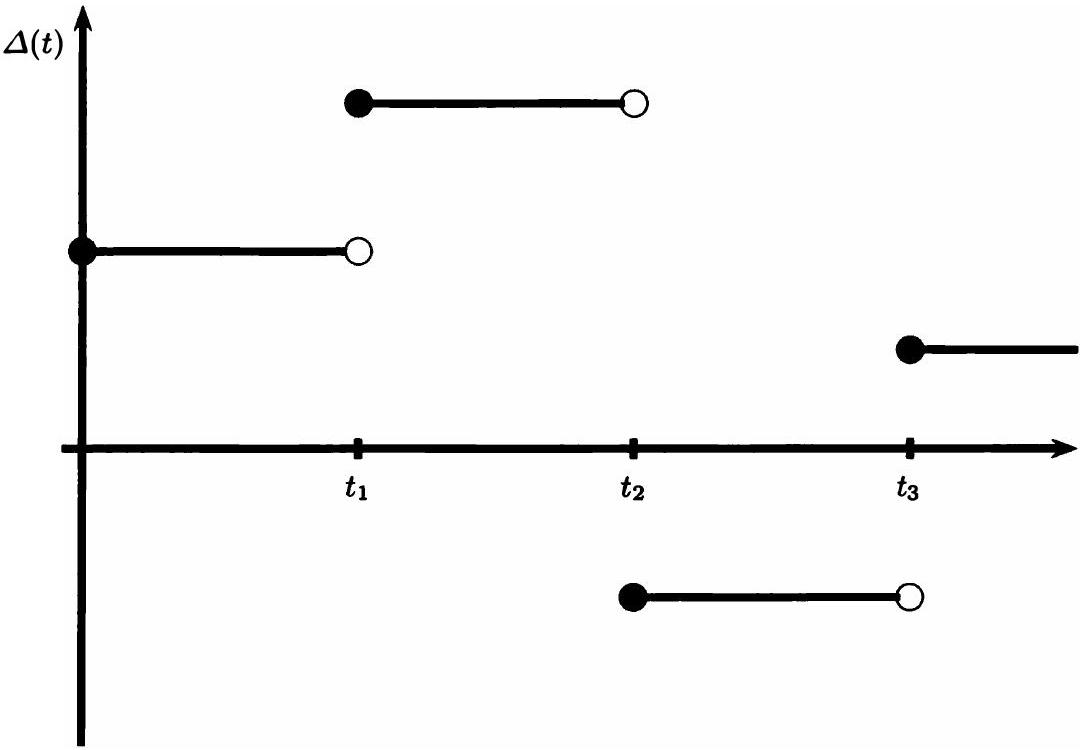
\includegraphics[width=\textwidth]{2024_03_27_8bb2f394a7b7e1201cbeg-03}
        \begin{tikzpicture}[scale=1.50]
            % Axes
            \draw[thick,->] (-0.5,0) -- (6,0) node[anchor=north] {$t$};
            \draw[thick,->] (0,-1.5) -- (0,2) node[anchor=east] {};
        
            % t1, t2, t3 markers on the axis
            \draw (1,1pt) -- (1,-3pt) node[anchor=north] {$t_1$};
            \draw (3,1pt) -- (3,-3pt) node[anchor=north] {$t_2$};
            \draw (5,1pt) -- (5,-3pt) node[anchor=north] {$t_3$};
        
            % Steps
            % Horizontal line from 0 to t1
            \draw[thick] (0,1) -- (1,1); % line segment
            \filldraw (0,1) circle (2pt); % filled circle at start
            \draw[thick] (1,1) circle (2pt); % the circle itself
            \filldraw[fill=white] (1,1) circle (2pt); % white filling
 
            % Horizontal line from t1 to t2
            \draw[thick] (1,1.5) -- (3,1.5);
            \filldraw (1,1.5) circle (2pt); 
            \draw[thick] (3,1.5) circle (2pt); 
            \filldraw[fill=white] (3,1.5) circle (2pt); 
            
             % Horizontal line from t2 to t3
            \draw[thick] (3,-0.75) -- (5,-0.75);
            \filldraw (3,-0.75) circle (2pt);
            \draw[thick] (5,-0.75) circle (2pt); 
            \filldraw[fill=white] (5,-0.75) circle (2pt); 
            
            % Horizontal line from t3 onward
            \draw[thick] (5,0.35) -- (6,0.35);
            \filldraw (5,0.35) circle (2pt); 

        \end{tikzpicture}

    \end{center}
    \caption{A path of a simple process.}
    \label{fig:simple_process}
\end{figure}

The \emph{Ito integral of a simple process} $\Delta(t)$ is defined by:
\begin{equation}
I(t):=\sum_{j=0}^{k-1} \Delta(t_{j})[W(t_{j+1})-W(t_{j})]+\Delta(t_{k})[W(t)-W(t_{k})] \label{eq:ito_integral_simple}
\end{equation}
which we write as
\begin{equation*}
I(t)=\int_{0}^{t} \Delta(u) dW(u).
\end{equation*}
In particular, we can take $t=t_{n}=T$, and (\ref{eq:ito_integral_simple}) provides a definition for the Ito integral (\ref{eq:ito_integral}). We have managed to define this integral not only for the upper limit of integration $T$ but also for every upper limit of integration $t$ between 0 and $T$.

\subsection{Properties of the Integral}\label{subsec:integral_properties}
The Ito integral (\ref{eq:ito_integral_simple}) is defined over the martingale $W(t)$. A martingale has no tendency to rise or fall, and hence it is to be expected that $I(t)$, thought of as a process in its upper limit of integration $t$, also has no tendency to rise or fall. We formalize this observation by the next theorem.
\begin{theorem}\label{thm:ito_integral_martingale}
The Ito integral defined by (\ref{eq:ito_integral_simple}) is a martingale.
\end{theorem}
\begin{proof} The proof is in Section \ref{subsec:ito_proofs}.\end{proof}

Because $I(t)$ is a martingale and $I(0)=0$, we have $\mathbb{E} I(t)=0$ for all $t \geq 0$. It follows that $\operatorname{Var}(I(t))=\mathbb{E} I^{2}(t)$, a quantity that can be evaluated by the formula in the next theorem.
\begin{theorem}[Ito isometry] \label{thm:ito_isometry}
The Ito integral defined by (\ref{eq:ito_integral_simple}) satisfies
\begin{equation*}
\mathbb{E} I^{2}(t)=\mathbb{E} \int_{0}^{t} \Delta^{2}(u) du.
\end{equation*}
\end{theorem}
\begin{proof} The proof is in Section \ref{subsec:ito_proofs}.\end{proof}

We turn to the quadratic variation of the Ito integral $I(t)$.
\begin{theorem}\label{thm:quadratic_variation}
The quadratic variation accumulated up to time $t$ by the Ito integral (\ref{eq:ito_integral_simple}) is
\begin{equation}
[I, I](t)=\int_{0}^{t} \Delta^{2}(u) du. \label{eq:quadratic_variation_formula}
\end{equation}
\end{theorem}
\begin{proof} The proof is in Section \ref{subsec:ito_proofs}.\end{proof}

In Theorems \ref{thm:ito_isometry} and \ref{thm:quadratic_variation}, we finally see how the quadratic variation and the variance of a process can differ. The quadratic variation is computed path-by-path, and the result can depend on the path. If along one path of the Brownian motion we have large values of $\Delta(u)$, the Ito integral will have a large quadratic variation. Along a different path, we could have small positions $\Delta(u)$ and the Ito integral would have a small quadratic variation. The quadratic variation can be regarded as a measure of risk, and it depends on the size of the positions we take. The variance of $I(t)$ is an average over all possible paths of the quadratic variation. Because it is the expectation of something, it cannot be random. We emphasize here that what we are calling variance is not the empirical variance. Empirical (or sample) variance is computed from a realized path and is an estimator of the theoretical variance we are discussing. The empirical variance is sometimes carelessly called variance, which creates the possibility of confusion.

The Ito integral formula $I(t)=\int_{0}^{t} \Delta(u) dW(u)$ can be written in differential form as $dI(t)=\Delta(t) dW(t)$. Similarly, the quadratic variation formula $[W,W](t)=t$, can be written in differential form as $dW(t) dW(t)=dt$. Thus, at least informally, we can square $dI(t)$:
\begin{equation}
dI(t) dI(t)=\Delta^{2}(t) dW(t) dW(t)=\Delta^{2}(t) dt
\end{equation}
This equation says that the Ito integral $I(t)$ accumulates quadratic variation at rate $\Delta^{2}(t)$ per unit time. 

\begin{remark}\label{rmk:differential_integral_forms}
Equations
\begin{equation}
I(t)=\int_{0}^{t} \Delta(u) d W(u)
\end{equation}
and
\begin{equation}
d I(t)=\Delta(t) d W(t) \label{eq:ito_differential_form}
\end{equation}
mean almost the same thing. The first equation has the precise meaning given by (\ref{eq:ito_integral_simple}). The second equation has the imprecise meaning that when we move forward a little bit in time from time $t$, the change in the Ito integral $I(t)$ is $\Delta(t)$ times the change in the Brownian motion $dW(t)$. It also has a precise meaning, which one obtains by integrating both sides, remembering to put in a constant of integration $I(0)$:
\begin{equation}
I(t)=I(0)+\int_{0}^{t} \Delta(u) dW(u) \label{eq:ito_integral_form}
\end{equation}
We say that the second is the differential form of the third and that the third is the integral form of the second. These two equations mean exactly the same thing.

The only difference between the second and third equations, and hence the only difference between the first and second, is that the first specifies the initial condition $I(0)=0$, whereas (\ref{eq:ito_differential_form}) and (\ref{eq:ito_integral_form}) permit $I(0)$ to be any arbitrary constant.
\end{remark}

\subsection{Ito's Integral for More General Integrands}
In this section, we define the Ito integral $\int_{0}^{T} \Delta(t) d W(t)$ for integrands $\Delta(t)$ that are allowed to vary continuously with time and also to jump. In particular, we no longer assume that $\Delta(t)$ is a simple process.

We do assume that $\Delta(t), t \geq 0$, is adapted to the filtration $\mathcal{F}(t), t \geq 0$. We also assume the mean-square-integrability condition
\begin{equation}
\mathbb{E} \int_{0}^{T} \Delta^{2}(t) d t<\infty
\end{equation}
In order to define $\int_{0}^{T} \Delta(t) d W(t)$, we approximate $\Delta(t)$ by simple processes. Figure \ref{fig:approximation} suggests how this can be done. In that figure, the continuously varying $\Delta(t)$ is shown as a solid red line and the approximating simple integrand is dashed. Notice that $\Delta(t)$ is allowed to jump. The approximating simple integrand is constructed by choosing a partition $0=t_{0}<t_{1}<t_{2}<t_{3}<t_{4}<t_{5}$, setting the approximating simple process equal to $\Delta(t_{j})$ at each $t_{j}$, and then holding the simple process constant over the subinterval $[t_{j}, t_{j+1})$. As the maximal step size of the partition approaches zero, the approximating integrand will become a better and better approximation of the continuously varying one.
\begin{figure}
    \begin{center}
        %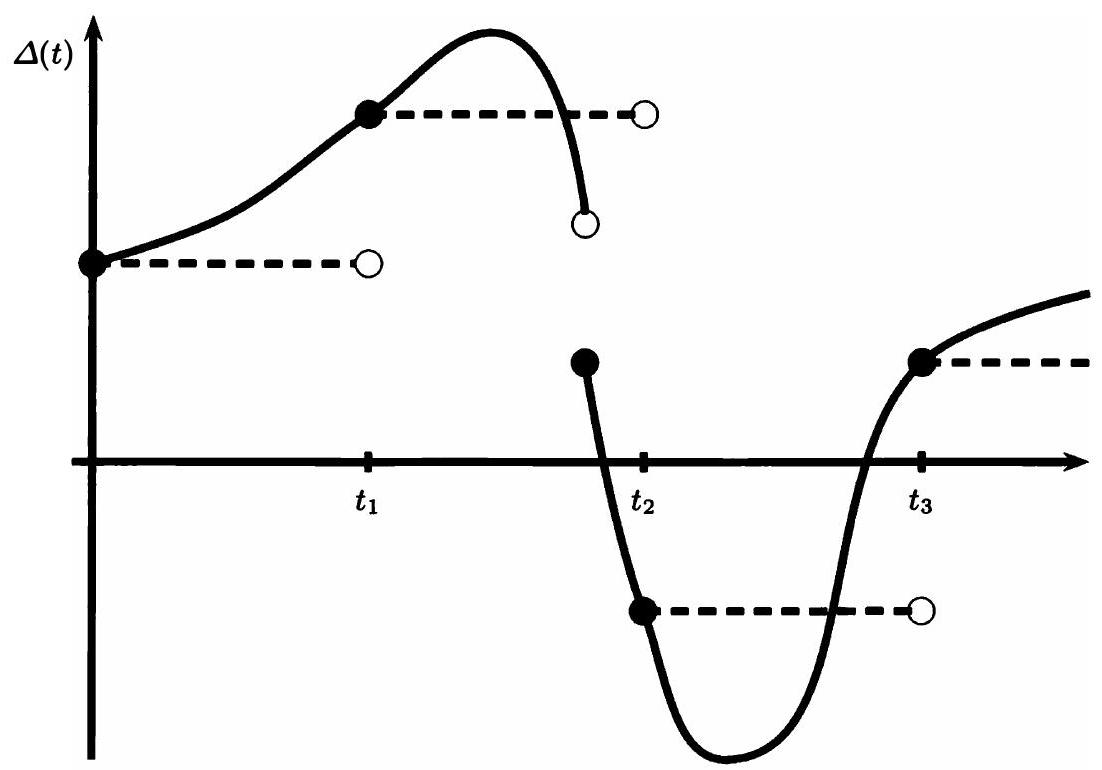
\includegraphics[width=\textwidth]{2024_03_27_8bb2f394a7b7e1201cbeg-09}
    \resizebox{.8\textwidth}{!}{
    \begin{tikzpicture}
      \riemannsum[-2.5:0.5:3]{
        function={\x}{sin(\x r)},
         line={thick, red, samples=300, domain=-2.5:0},
        left={thick, fill=none},
        right={draw=none},
       axis={draw=none},
        yshift=-1cm,
        xshift=-1cm,
      }                                        
      \riemannsum[0.5:2.5:2]{
        function={\x}{sin(2*\x r) + cos(\x^2/3.5 r)},
         line={thick, red, samples=300, domain=0:2},
        left={thick, fill=none},
        right={draw=none},
            axis={draw=none},
        yshift=-1.5cm,
        xshift=-1cm,
      }
      \pgfonlayer{left}
            \node [circle, color = black,
                             draw,
                             fill = white,
                             line width = 0.3pt,
                             inner xsep = 0pt,
                             inner ysep = 0pt,
                             minimum size=3pt,
                             solid]  at (-1,-1) {};
       
            \node [circle, color = black,
                             draw,
                             fill = black,
                             line width = 0.3pt,
                             inner xsep = 0pt,
                             inner ysep = 0pt,
                             minimum size=3pt,
                             solid]  at (-1,-0.5) {};             
                             
            \draw[gray!15,step=1cm] (-4,-4) grid (2,2);    
            \draw[line width=0.5mm, -latex] (-4,-2.5) -- (2.2,-2.5) node[right] {$t$};
            %\foreach \x in {-4,...,2} \draw (\x,.1)--(\x,-.1) node[below] {\footnotesize $\x$};
            \draw[line width=0.5mm,  -latex] (-3.5,-2.8) -- (-3.5,1.2) node[above] {$\Delta(t)$};
               
            
 	\foreach \x in {1,...,5} \draw (\x-3.5,.1-2.5)--(\x-3.5,-.1-2.5) node[below] {\footnotesize $t_\x$};

  
        \endpgfonlayer
    \end{tikzpicture}


    }
    \end{center}
    \caption{ Approximating a continuously varying integrand.}
    \label{fig:approximation}
\end{figure}

In general, then, it is possible to choose a sequence $\Delta_{n}(t)$ of simple processes such that as $n \rightarrow \infty$ these processes converge to the continuously varying $\Delta(t)$. By ``converge'', we mean that
\begin{equation*}
\lim _{n \rightarrow \infty} \mathbb{E} \int_{0}^{T}\left|\Delta_{n}(t)-\Delta(t)\right|^{2} dt=0.
\end{equation*}

For each $\Delta_{n}(t)$, the Ito integral $\int_{0}^{t} \Delta_{n}(u) d W(u)$ has already been defined for $0 \leq t \leq T$. We define the Ito integral for the continuously varying integrand $\Delta(t)$ by the formula
\begin{equation*}
\int_{0}^{t} \Delta(u) d W(u)=\lim _{n \rightarrow \infty} \int_{0}^{t} \Delta_{n}(u) d W(u), \quad 0 \leq t \leq T
\end{equation*}
This integral inherits the properties of Ito integrals of simple processes:
\begin{enumerate}[label=(\roman*)]
    \item (Continuity) As a function of the upper limit of integration $t$, the paths of $I(t)$ are continuous.
    
    \item (Adaptivity) For each $t, I(t)$ is $\mathcal{F}(t)$-measurable.
    
    \item (Linearity) If $I(t)=\int_{0}^{t} \Delta(u) d W(u)$ and $J(t)=\int_{0}^{t} \Gamma(u) d W(u)$, then $I(t) \pm J(t)=\int_{0}^{t}(\Delta(u) \pm \Gamma(u)) d W(u)$; furthermore, for every constant $c$, $c I(t)=\int_{0}^{t} c \Delta(u) d W(u)$.
    
    \item (Martingale) $I(t)$ is a martingale.
    
    \item (Ito isometry) $\mathbb{E} I^{2}(t)=\mathbb{E} \int_{0}^{t} \Delta^{2}(u) d u$.
    
    \item (Quadratic variation) $[I, I](t)=\int_{0}^{t} \Delta^{2}(u) d u$.
    \end{enumerate}

\subsection{Square Integrable Functions}
We have defined the Ito integral $\int_{0}^{T} \Delta^{2}(t) dW(t)$ under the square-integrability condition. It turns out that many economically interesting trading strategies do not fall into the class. The integral can be defined under the weaker condition (without the expectation)
\begin{equation*}
\int_{0}^{T} \Delta^{2}(t)dt<\infty, \quad \text{ almost surely },
\end{equation*}
i.e., $\Delta (t) \in L^{2}(\mathcal{F})$,
but then the integral is not guaranteed to be a martingale, but a \textit{local martingale}, a much weaker property. We usually impose restrictions on  $\Delta (t)$ so that it is still in $L^{2}(\mathcal{F})$ but so that the Ito integral is a martingale.





\subsection{Ito Processes}
Now we can define the process in equation (\ref{eq:general_diffusion}) more precisely. A \emph{diffusion process} or \emph{Ito process} is a process $S$ in $\mathbb{R}$ such that
\begin{equation}
S_{t}=S_{0}+\int_{0}^{t} \mu_{s} ds+\int_{0}^{t} \sigma_{s} dZ_{s} \label{eq:ito_process}
\end{equation}
where the process $\mu \in \mathcal{L}^{1}$ and the process $\sigma \in \mathcal{L}^{2}$.

An Ito process is the sum of a ``normal'' (non-stochastic) integral and a stochastic integral. A Brownian motion is obviously an Ito process.

We frequently write an Ito process in ``differential'' form, as in equation (\ref{eq:general_diffusion}),
\begin{equation}
dS_{t}=\mu_{t} dt+\sigma_{t} dZ_{t}, \label{eq:ito_process_differential}
\end{equation}
and refer to $dS_{t}$ as the \emph{increment} of $S$ at time $t$. If $\mu$, $\sigma$ are mean-square integrable then
\begin{equation}
\left.\frac{d}{d \tau} E_{t}\left(S_{\tau}\right)\right|_{\tau=t}=\mu_{t}, \quad \text { a.s. }
\end{equation}
and
\begin{equation}
\left.\frac{d}{d \tau} \operatorname{Var}_{t}\left(S_{\tau}\right)\right|_{\tau=t}=\sigma_{t}^{2}, \quad \text { a.s. }
\end{equation}

We frequently write these equations as $E(dS_{t})=\mu_{t} dt$ and $\operatorname{Var}(dS_{t})=\sigma_{t}^{2} dt$, respectively, and refer to $\mu_{t} dt$ as the \emph{mean} of $dS_{t}$, and $\sigma_{t}^{2} dt$ as its \emph{variance}. We refer to the process $\mu$ as the \emph{drift process} and to the process $\sigma$ as the \emph{diffusion process}.

\subsection{Ito's Lemma}
We now restate Ito's Lemma more formally:
\begin{theorem}\label{thm:ito_lemma}[Ito's Lemma - One-Dimensional Case]
Suppose that $S$ is an Ito process with
\begin{equation*}
dS_{t}=\mu_{t} d t+\sigma_{t} dZ_{t}
\end{equation*}
and $f: \mathbb{R}^{2} \rightarrow \mathbb{R}$ is twice continuously differentiable. Then the process $C$ defined by $C_{t}=f\left(t, S_{t}\right)$ is an Ito process with
\begin{equation*}
d C_{t}=\left(\mathcal{D}_{S} f\left(t, S_{t}\right)+f_{t}\left(t, S_{t}\right)\right) d t+f_{S}\left(t, S_{t}\right) \sigma_{t} d Z_{t}
\end{equation*}
where
\begin{equation*}
\mathcal{D}_{S} f\left(t, S_{t}\right)=f_{S}\left(t, S_{t}\right) \mu_{t}+\frac{1}{2} f_{S S}\left(t, S_{t}\right) \sigma_{t}^{2}
\end{equation*}
\end{theorem}
As mentioned earlier, Ito's lemma extends the chain rule of calculus for stochastic integrals. If the process $S$ was just a non-stochastic integral
\begin{equation*}
d S_{t}=\mu_{t} dt
\end{equation*}
then the chain rule of calculus would imply that
\begin{equation*}
d C_{t}=f_{S}(t, S_{t}) d S_{t}+f_{t}(t, S_{t}) d t=[f_{S}(t, S_{t}) \mu_{t}+f_{t}(t, S_{t})] dt.
\end{equation*}
When, however, $S$ includes a stochastic integral, it is not true that
\begin{equation*}
d C_{t}=f_{S}(t, S_{t}) d S_{t}+f_{t}(t, S_{t}) d t
\end{equation*}
because this would omit the term
\begin{equation*}
\frac{1}{2} f_{S S}\left(t, S_{t}\right) \sigma_{t}^{2} d t
\end{equation*}

\subsection{Ito's Lemma for Two Variables}
Suppose $X$ and $Y$ are Ito processes with differentials
\begin{align}
d X(t) & =\Theta_{1}(t) d t+\sigma_{11}(t) d W_{1}(t)+\sigma_{12}(t) d W_{2}(t)  \label{4.8.6}\\
d Y(t) & =\Theta_{2}(t) d t+\sigma_{21}(t) d W_{1}(t)+\sigma_{22}(t) d W_{2}(t)
 \label{4.8.7}
\end{align}
where $W_{1}$ and $W_{2}$ are independent Brownian motions. Then
\begin{align}
d X(t) d X(t) & =\left(\sigma_{11}^{2}(t)+\sigma_{12}^{2}(t)\right) d t  \label{4.8.8}\\
d X(t) d Y(t) & =\left(\sigma_{11}(t) \sigma_{21}(t)+\sigma_{12}(t) \sigma_{22}(t)\right) d t  \label{4.8.9}\\
d Y(t) d Y(t) & =\left(\sigma_{21}^{2}(t)+\sigma_{22}^{2}(t)\right) d t
\label{4.8.10}
\end{align} 

Equations (\ref{4.8.8})-(\ref{4.8.10}) can be obtained by multiplying the equations (\ref{4.8.6}) and (\ref{4.8.7}) for $dX(t)$ and $dY(t)$ and using the multiplication table
\begin{align*}
d W_{i}(t) d W_{i}(t)&=d t,\\
d W_{i}(t) d t&=d t d W_{i}(t)=0,\\
d t d t=0,
\end{align*}
and
\begin{equation}
d W_{1}(t) d W_{2}(t)=0. \label{4.8.11}
\end{equation}
Equation (\ref{4.8.11}) holds for independent Brownian motions. If instead we had
\begin{equation*}
d W_{1}(t) d W_{2}(t)=\rho d t
\end{equation*}
for a constant $\rho \in[-1,1]$, then $\rho$ would be the correlation between $W_{1}(t)$ and $W_{2}(t)$ (i.e., $\left.\mathbb{E}\left[W_{1}(t) W_{2}(t)\right]=\rho t\right)$.

Now suppose $f(t, x, y)$ is a function of the time variable $t$ and two dummy variables $x$ and $y$. The Ito-Doeblin formula is now
\begin{align}
& d f(t, X(t), Y(t)) \notag \\
& =f_{t}(t, X(t), Y(t)) d t+f_{x}(t, X(t), Y(t)) d X(t)+f_{y}(t, X(t), Y(t)) d Y(t) \notag\\
& \quad \frac{1}{2} f_{x x}(t, X(t), Y(t)) d X(t) d X(t)+f_{x y}(t, X(t), Y(t)) d X(t) d Y(t) \notag\\
& \quad+\frac{1}{2} f_{y y}(t, X(t), Y(t)) d Y(t) d Y(t).
\label{4.8.12}
\end{align}
Replacing all the differentials on the right-hand side of (\ref{4.8.12}) by their formulas (\ref{4.8.6})-(\ref{4.8.10}) and integrating, one obtains a formula for the stochastic process $f(t, X(t), Y(t))$ as the sum of $f(0, X(0), Y(0))$, an ordinary integral with respect to time, an Ito integral with respect to $dW_{1}$, and an Ito integral with respect to $dW_{2}$.

Equation (\ref{4.8.12}) gives us Ito's product rule:
\begin{equation*}
d(X(t) Y(t))=X(t) d Y(t)+Y(t) d X(t)+d X(t) d Y(t)
\end{equation*}
The analogous rule for non-stochastic differentials, $d(X(t) Y(t))=X(t) d Y(t)+Y(t) d X(t)$, omits the term $dX(t) dY(t)$. When $dX(t)$ and $dY(t)$ are not stochastic, the term $dX(t) dY(t)$ is of order $dt^2$ and can be ignored. Instead, when $dX(t)$ and $dY(t)$ are stochastic the term $dX(t) dY(t)$ is of order $dt$ and cannot be ignored.


% \subsection{Conditional Moments of Diffusion Processes}
% There are many situations when one needs to compute conditional moments of diffusion processes. For instance, we may want to know expected returns and variances of returns on financial assets over finite time intervals. Or we may want to use the method of moments (GMM) to estimate a diffusion process from discretely sampled data. Or we may want to compute prices of derivative assets, which typically boils down to computing moments of diffusion processes. We now introduce a useful tool for computing conditional expectations of functions of diffusion processes.

% We will gloss over the technicalities. One can find precise technical conditions and further references in Duffie (Appendix E) and Oksendal (Chapter 8.1).

% Consider a diffusion process $X_{t}$ with coefficients $\mu(t, X)$ and $\sigma(t, X)$. Our task is to compute a conditional expectation $f(t, x)=E\left[g\left(X_{T}\right) \mid X_{t}=x\right]$. Proceeding heuristically, suppose that the conditional expectation is a sufficiently smooth function of $t$ and $x$. By the law of iterated expectations, $f\left(t, X_{t}\right)=E_{t}\left[f\left(t+d t, X_{t+d t}\right)\right]$, therefore $E_{t}\left[d f\left(t, X_{t}\right)\right]=0$.

% Using Ito's Lemma,
% \begin{equation*}
% E_{t}\left[d f\left(t, X_{t}\right)\right]=\left(\mathcal{D}_{X} f\left(t, X_{t}\right)+f_{t}\left(t, X_{t}\right)\right) d t=0 .
% \end{equation*}
% Thus, we see that the conditional expectation $f(t, x)$ must satisfy a partial differential equation (PDE)
% \begin{equation*}
% f_{t}+\mu(t, x) f_{x}+\frac{1}{2} \sigma(t, x)^{2} f_{x x}=0 \label{2.6.7}
% \end{equation*}
% with the boundary condition
% \begin{equation*}
% f(T, x)=g(x) . \label{2.6.8}
% \end{equation*}
% The above equation is called Kolmogorov's backward equation.

% Kolmogorov's backward equation can be a useful tool for estimating diffusion processes from discretely sampled data. Suppose we observe realizations $X_{n}, n=0,1, \ldots N$ of the diffusion process $X_{t}$. Assume furthermore that the diffusion coefficients are known in a parametric form: $\mu(t, X ; \theta)$ and $\sigma(t, X ; \theta)$. A standard method of estimating unknown distribution parameters is by maximum likelihood, but for that we must know the conditional transition density $p\left(X_{n}, X_{n+1} ; \theta\right)$ for the process $X_{t}$. Here, $p(x, y ; \theta)$ is the density of the distribution of $y=X_{n+1}$ conditional on $X_{n}=x$.

% Example 2.6.4 As an example, we compute the transition density of the Ornstein-Uhlenbeck process
% \begin{equation*}
% d X_{t}=-\lambda\left(X_{t}-\bar{X}\right) d t+\sigma d Z_{t}
% \end{equation*}
% To characterize the transition density, we compute the characteristic function
% \begin{equation*}
% \phi(x, w)=E\left[e^{i w X_{T}} \mid X_{0}=x\right], \quad i=\sqrt{-1}
% \end{equation*}
% Define
% \begin{equation*}
% f(t, x ; w)=E\left[e^{i w X_{T}} \mid X_{t}=x\right]
% \end{equation*}
% Then the characteristic function is given by $\phi(x, w)=f(0, x)$. The function $f(t, x)$ satisfies the Kolmogorov's backward equation:
% \begin{equation*}
% f_{t}-f_{x} \lambda(x-\bar{X})+f_{x x} \frac{\sigma^{2}}{2}=0, \quad f(T, x)=e^{i w x} . \label{2.6.9}
% \end{equation*}
% We look for the solution in the form $f(t, x)=\exp \left[a_{0}(t)+a_{1}(t) x\right]$. Substituting this into (2.6.9), we derive a system of ODEs on the coefficients $a_{0}, a_{1}$:
% \begin{align}
% \dot{a}_{0} & =\lambda \bar{X} a_{1}+\frac{\sigma^{2}}{2} a_{1}^{2}, \quad a_{0}(T)=0,  \label{2.6.10}\\
% \dot{a}_{1} & =\lambda a_{1}, \quad a_{1}(T)=i w .
%  \label{2.6.11}
% \end{align}
% Integrating the above system of ODEs, we find
% \begin{align}
% & a_{0}(0)=i w e^{-\lambda T} .  \label{2.6.12}\\
% & a_{1}(0)=i w \bar{X}\left(1-e^{-\lambda T}\right)-w^{2} \frac{\sigma^{2}}{4 \lambda}\left(1-e^{-2 \lambda T}\right) .
% \label{2.6.13}
% \end{align}
% Thus, we know the characteristic function of the transition density:
% \begin{equation*}
% \phi(x, w)=\exp \left[i w\left(\bar{X}+(x-\bar{X}) e^{-\lambda T}\right)-w^{2} \frac{\sigma^{2}}{4 \lambda}\left(1-e^{-2 \lambda T}\right)\right] .
% \end{equation*}
% Remember that the characteristic function of a Normal random variable $\mathcal{N}\left(\mu, \sigma^{2}\right)$ is given by $\exp \left[i w \mu-w^{2} \frac{\sigma^{2}}{2}\right]$. We conclude that our transition density is Gaussian with mean $\bar{X}+(x-$ $\bar{X}) e^{-\lambda T}$ and variance $\frac{\sigma^{2}}{2 \lambda}\left(1-e^{-2 \lambda T}\right)$, where $T$ is the time between successive observations of the process $X_{t}$.

\section{Change of Measure}
\begin{theorem}[Girsanov's Theorem]\label{thm: thm_273} 
Consider a process $\eta \in\left(\mathcal{L}^{2}\right)^{d}$ such that $\xi^{\eta}$ is a martingale. Then the process $Z^{\eta}$ defined by
\begin{equation}
Z_{t}^{\eta}=Z_{t}+\int_{0}^{t} \eta_{s} d s \label{2.7.3}
\end{equation}
is a Brownian motion under $Q^{\eta}$.
$Z^{\eta}$ has a martingale representation property under $Q^{\eta}$ : for any local $Q^{\eta}$-martingale $M_{t}$, adapted to $\mathbb{F}$, there exists a process $\phi \in\left(\mathcal{L}^{2}\right)^{d}$, such that
\begin{equation*}
M_{t}=M_{0}+\int_{0}^{t} \phi_{s} d Z_{s}^{\eta}
\end{equation*}
\end{theorem}
Girsanov's theorem says that, by adding a drift to a process that is a Brownian motion under the probability measure $P$, we can obtain a process that is a Brownian motion under the probability measure $Q^{\eta}$. To understand intuitively why the process $Z^{\eta}$ has no drift, we consider the increment
\begin{equation*}
d Z_{t}^{\eta}=d Z_{t}+\eta_{t} d t
\end{equation*}
In addition, we think of the increment $d Z_{t}$ as taking the values $\sqrt{d t}$ and $-\sqrt{d t}$. Under $P$, the probability of each value (conditional on time $t$ ) is $1 / 2$. Under $Q^{\eta}$, the probability of $\sqrt{d t}$ is
\begin{equation*}
\left.\frac{1}{2} \frac{\xi_{t+d t}^{\eta}}{\xi_{t}^{\eta}}\right|_{d Z_{t}=\sqrt{d t}}=\frac{1}{2} \exp \left(-\eta_{t} \sqrt{d t}\right)+o(\sqrt{d t})
\end{equation*}
and the probability of $-\sqrt{d t}$ is
\begin{equation*}
\frac{1}{2} \exp \left(\eta_{t} \sqrt{d t}\right)+o(\sqrt{d t})
\end{equation*}

Therefore, the expectation of $d Z_{t}^{\eta}$ is
\begin{equation*}
\begin{aligned}
& \frac{1}{2} \exp \left(-\eta_{t} \sqrt{d t}\right)\left(\sqrt{d t}+\eta_{t} d t\right)+\frac{1}{2} \exp \left(\eta_{t} \sqrt{d t}\right)\left(-\sqrt{d t}+\eta_{t} d t\right)+o(d t) \\
= & \frac{1}{2}\left(1-\eta_{t} \sqrt{d t}\right)\left(\sqrt{d t}+\eta_{t} d t\right)+\frac{1}{2}\left(1+\eta_{t} \sqrt{d t}\right)\left(-\sqrt{d t}+\eta_{t} d t\right)+o(d t) .
\end{aligned}
\end{equation*}
This is equal to 0 in order $dt$.

Girsanov's theorem has the following important implication.

\begin{proposition}\label{prop: prop_271}
Consider an Ito process $S$ in $\mathbb{R}^{N}$,
\begin{equation*}
S_{t}=S_{0}+\int_{0}^{t} \mu_{s} d s+\int_{0}^{t} \sigma_{s} d Z_{s}
\end{equation*}
and processes $\nu \in\left(\mathcal{L}^{1}\right)^{N}$ and $\eta \in\left(\mathcal{L}^{2}\right)^{d}$ such that
\begin{equation*}
\sigma_{t} \eta_{t}=\mu_{t}-\nu_{t}
\end{equation*}
If the process $\xi^{\eta}$ is a martingale, then $S$ is an Ito process under $Q^{\eta}$, and
\begin{equation*}
S_{t}=S_{0}+\int_{0}^{t} \nu_{s} d s+\int_{0}^{t} \sigma_{s} d Z_{s}^{\eta}
\end{equation*}
\end{proposition}
We can thus write an Ito process $S$ under $P$ as an Ito process under $Q^{\eta}$. The drift changes, but the diffusion stays the same.

In fact, the reverse is true: we can show that under any equivalent probability measure w.r.t. which $S$ is a martingale, the diffusion part of the process $S_{t}$ stays the same, and only the drift changes.

\section{Summary}
Let $W(t)$ be a Brownian motion and $\Delta(t)$ a stochastic process adapted to the filtration of the Brownian motion. The Ito integral
\begin{equation*}
I(t)=\int_{0}^{t} \Delta(u) d W(u) \label{4.8.1}
\end{equation*}
is a martingale. Because it is zero at time $t=0$, its expectation is zero for all $t$. 
% More generally, if for $t \leq s$ we define
% \begin{equation*}
% I_t(s) = \int_{t}^{s} \Delta(u) dW(u),
% \end{equation*}
% then the martingale property of the Ito integral implies that
% \begin{align*}
% E_t[I_t(s)] &= I_t(t)\\
% &= E_t\left[\int_{t}^{t} \Delta(u) dW(u) \right]\\
% &=0.
% \end{align*}
% In differential form, the last equation gives
% \begin{align*}
% E_t[dW(s)] &= 0
% \end{align*}

Its variance is given by Ito's isometry
\begin{equation*}
\mathbb{E} I^{2}(t)=\mathbb{E} \int_{0}^{t} \Delta^{2}(u) d u \label{4.8.2}
\end{equation*}
An Ito process is a process of the form
\begin{equation*}
X(t)=X(0)+\int_{0}^{t} \Delta(u) d W(u)+\int_{0}^{t} \Theta(u) d u \label{4.8.4}
\end{equation*}
where $X(0)$ is nonrandom and $\Delta(u)$ and $\Theta(u)$ are adapted stochastic processes. In differential notation, we write
\begin{equation*}
d X(t)=\Delta(t) d W(t)+\Theta(t) d t
\end{equation*}
To compute expressions in differential form, we use the multiplication table
\begin{equation*}
d W(t) d W(t)=d t, \quad d W(t) d t=d t d W(t)=0, \quad d t d t=0
\end{equation*}
For example,
\begin{align*}
dX(t) dX(t) & =(\Delta(t) dW(t)+\Theta(t) dt)^{2} \\
& =\Delta^{2}(t) dW(t) dW(t)+2 \Delta(t) \Theta(t) dW(t) dt+\Theta^{2}(t) dt dt \\
& =\Delta^{2}(t) dt
\end{align*}
Let $f(t, x)$ is a function of the time variable $t$ and a stochastic process $x$. The Ito-Doeblin formula is
\begin{align*}
    df(t, X(t))=f_{t}(t, X(t)) d t+f_{x}(t, X(t)) d X(t)+\frac{1}{2} f_{x x}(t, X(t)) dX(t) dX(t).
\end{align*}

For two stochastic processes $X(t)$ and $Y(t)$, Ito's product rule is
\begin{equation*}
d(X(t) Y(t))=X(t) d Y(t)+Y(t) d X(t)+d X(t) d Y(t).
\end{equation*}
\begin{optional}
\subsection{Proofs}\label{subsec:ito_proofs}

\begin{proof}[Proof of Theorem \ref{thm:ito_integral_martingale}]
Let $0 \leq s \leq t \leq T$ be given. We shall assume that $s$ and $t$ are in different subintervals of the partition $\Pi$ (i.e., there are partition points $t_{\ell}$ and $t_{k}$ such that $t_{\ell}<t_{k}, s \in\left[t_{\ell}, t_{\ell+1}\right)$, and $\left.t \in\left[t_{k}, t_{k+1}\right)\right)$. If $s$ and $t$ are in the same subinterval, the following proof simplifies. The Ito integral may be rewritten as
\begin{align}
& I(t)=\sum_{j=0}^{\ell-1} \Delta\left(t_{j}\right)\left[W\left(t_{j+1}\right)-W\left(t_{j}\right)\right]+\Delta\left(t_{\ell}\right)\left[W\left(t_{\ell+1}\right)-W\left(t_{\ell}\right)\right] \\
& \quad+\sum_{j=\ell+1}^{k-1} \Delta\left(t_{j}\right)\left[W\left(t_{j+1}\right)-W\left(t_{j}\right)\right]+\Delta\left(t_{k}\right)\left[W(t)-W\left(t_{k}\right)\right]
\label{4.2.3}
\end{align}
We must show that $\mathbb{E}[I(t) \mid \mathcal{F}(s)]=I(s)$. We take the conditional expectation of each of the four terms on the right-hand side. Every random variable in the first sum $\sum_{j=0}^{\ell-1} \Delta\left(t_{j}\right)\left[W\left(t_{j+1}\right)-W\left(t_{j}\right)\right]$ is $\mathcal{F}(s)$-measurable because the latest time appearing in this sum is $t_{\ell}$ and $t_{\ell} \leq s$. Therefore,
\begin{equation}
\mathbb{E}\left[\sum_{j=0}^{\ell-1} \Delta\left(t_{j}\right)\left[W\left(t_{j+1}\right)-W\left(t_{j}\right)\right] \mid \mathcal{F}(s)\right]=\sum_{j=0}^{\ell-1} \Delta\left(t_{j}\right)\left[W\left(t_{j+1}\right)-W\left(t_{j}\right)\right]. \label{4.2.4}
\end{equation}
For the second term on the right-hand side, we use the properties of expectations and the martingale property of $W$ to write
\begin{align}
\mathbb{E}\left[\Delta\left(t_{\ell}\right)\left(W\left(t_{\ell+1}\right)-W\left(t_{\ell}\right)\right) \mid \mathcal{F}(s)\right] & =\Delta\left(t_{\ell}\right)\left(\mathbb{E}\left[W\left(t_{\ell+1}\right) \mid \mathcal{F}(s)\right]-W\left(t_{\ell}\right)\right) \\
& =\Delta\left(t_{\ell}\right)\left(W(s)-W\left(t_{\ell}\right)\right)
\label{4.2.5}
\end{align}
Adding these results, we obtain $I(s)$.

It remains to show that the conditional expectations of the third and fourth terms on the right-hand side are zero. We will then have $\mathbb{E}[I(t) \mid \mathcal{F}(s)]=I(s)$.

The summands in the third term are of the form $\Delta\left(t_{j}\right)\left[W\left(t_{j+1}\right)-W\left(t_{j}\right)\right]$, where $t_{j} \geq t_{\ell+1}>s$. This permits us to use the law of iterated expectations
\begin{align*}
\mathbb{E}\left\{\Delta\left(t_{j}\right)\right. & \left.\left(W\left(t_{j+1}\right)-W\left(t_{j}\right)\right) \mid \mathcal{F}(s)\right\} \\
& =\mathbb{E}\left\{\mathbb{E}\left[\Delta\left(t_{j}\right)\left(W\left(t_{j+1}\right)-W\left(t_{j}\right)\right) \mid \mathcal{F}\left(t_{j}\right)\right] \mid \mathcal{F}(s)\right\} \\
& =\mathbb{E}\left\{\Delta\left(t_{j}\right)\left(\mathbb{E}\left[W\left(t_{j+1}\right) \mid \mathcal{F}\left(t_{j}\right)\right]-W\left(t_{j}\right)\right) \mid \mathcal{F}(s)\right\} \\
& =\mathbb{E}\left\{\Delta\left(t_{j}\right)\left(W\left(t_{j}\right)-W\left(t_{j}\right)\right) \mid \mathcal{F}(s)\right\}=0
\end{align*}
At the end, we have used the fact that $W$ is a martingale. Because the conditional expectation of each of the summands in the third term on the right-hand side is zero, the conditional expectation of the whole term is zero:
\begin{equation*}
\mathbb{E}\left\{\sum_{j=\ell+1}^{k-1} \Delta\left(t_{j}\right)\left[W\left(t_{j+1}\right)-W\left(t_{j}\right)\right] \mid \mathcal{F}(s)\right\}=0
\end{equation*}
The fourth term on the right-hand side is treated like the summands in the third term, with the result that
\begin{align*}
\mathbb{E}\left\{\Delta\left(t_{k}\right)\right. & \left.\left(W(t)-W\left(t_{k}\right)\right) \mid \mathcal{F}(s)\right\} \\
& =\mathbb{E}\left\{\mathbb{E}\left[\Delta\left(t_{k}\right)\left(W(t)-W\left(t_{k}\right)\right) \mid \mathcal{F}\left(t_{k}\right)\right] \mid \mathcal{F}(s)\right\} \\
& =\mathbb{E}\left\{\Delta\left(t_{k}\right)\left(\mathbb{E}\left[W(t) \mid \mathcal{F}\left(t_{k}\right)\right]-W\left(t_{k}\right)\right) \mid \mathcal{F}(s)\right\} \\
& =\mathbb{E}\left\{\Delta\left(t_{k}\right)\left(W\left(t_{k}\right)-W\left(t_{k}\right)\right) \mid \mathcal{F}(s)\right\}=0 .
\end{align*}
\end{proof}

\begin{proof}[Proof of Theorem \ref{thm:ito_isometry}]
To simplify the notation, we set $D_{j}=W\left(t_{j+1}\right)-W\left(t_{j}\right)$ for $j=$ $0, \ldots, k-1$ and $D_{k}=W(t)-W\left(t_{k}\right)$ so that the Ito integral may be written as $I(t)=$ $\sum_{j=0}^{k} \Delta\left(t_{j}\right) D_{j}$ and
\begin{equation*}
I^{2}(t)=\sum_{j=0}^{k} \Delta^{2}\left(t_{j}\right) D_{j}^{2}+2 \sum_{0 \leq i<j \leq k} \Delta\left(t_{i}\right) \Delta\left(t_{j}\right) D_{i} D_{j}
\end{equation*}
We first show that the expected value of each of the cross terms is zero. For $i<$ $j$, the random variable $\Delta\left(t_{i}\right) \Delta\left(t_{j}\right) D_{i}$ is $\mathcal{F}\left(t_{j}\right)$-measurable, while the Brownian increment $D_{j}$ is independent of $\mathcal{F}\left(t_{j}\right)$. Furthermore, $\mathbb{E} D_{j}=0$. Therefore,
\begin{align*}
\mathbb{E}\left[\Delta\left(t_{i}\right) \Delta\left(t_{j}\right) D_{i} D_{j}\right]&=\mathbb{E}\left[\Delta\left(t_{i}\right) \Delta\left(t_{j}\right) D_{i}\right] \cdot \mathbb{E} D_{j}\\
&=\mathbb{E}\left[\Delta\left(t_{i}\right) \Delta\left(t_{j}\right) D_{i}\right] \cdot 0\\
&=0
\end{align*}
We next consider the square terms $\Delta^{2}\left(t_{j}\right) D_{j}^{2}$. The random variable $\Delta^{2}\left(t_{j}\right)$ is $\mathcal{F}\left(t_{j}\right)$- measurable, and the squared Brownian increment $D_{j}^{2}$ is independent of $\mathcal{F}\left(t_{j}\right)$. Furthermore, $\mathbb{E} D_{j}^{2}=t_{j+1}-t_{j}$ for $j=0, \ldots, k-1$ and $\mathbb{E} D_{k}^{2}=t-t_{k}$. Therefore,
\begin{align}
\mathbb{E} I^{2}(t) & =\sum_{j=0}^{k} \mathbb{E}\left[\Delta^{2}\left(t_{j}\right) D_{j}^{2}\right]\\
&=\sum_{j=1}^{k} \mathbb{E} \Delta^{2}\left(t_{j}\right) \cdot \mathbb{E} D_{j}^{2} \\
& =\sum_{j=0}^{k-1} \mathbb{E} \Delta^{2}\left(t_{j}\right)\left(t_{j+1}-t_{j}\right)+\mathbb{E} \Delta^{2}\left(t_{k}\right)\left(t-t_{k}\right)
\label{4.2.7}
\end{align}
But $\Delta\left(t_{j}\right)$ is constant on $\left[t_{j}, t_{j+1}\right)$, so
\[
\Delta^{2}(t_{j})(t_{j+1}-t_{j})=\int_{t_{j}}^{t_{j+1}} \Delta^{2}(u)\, d u.
\]
Similarly,
\[
\Delta^{2}(t_{k})(t-t_{k})=\int_{t_{k}}^{t} \Delta^{2}(u)\, d u.
\]
We may thus continue to obtain
\begin{align*}
\mathbb{E} I^{2}(t) & =\sum_{j=0}^{k-1} \mathbb{E} \int_{t_{j}}^{t_{j+1}} \Delta^{2}(u) d u+\mathbb{E} \int_{t_{k}}^{t} \Delta^{2}(u) d u \\
& =\mathbb{E}\left[\sum_{j=0}^{k-1} \int_{t_{j}}^{t_{j+1}} \Delta^{2}(u) d u+\int_{t_{k}}^{t} \Delta^{2}(u) d u\right]=\mathbb{E} \int_{0}^{t} \Delta^{2}(u) du.
\end{align*}
\end{proof}

\begin{proof}[Proof of Theorem \ref{thm:quadratic_variation}]
We first compute the quadratic variation accumulated by the Ito integral on one of the subintervals $\left[t_{j}, t_{j+1}\right]$ on which $\Delta(u)$ is constant. For this, we choose partition points
\begin{equation*}
t_{j}=s_{0}<s_{1}<\cdots<s_{m}=t_{j+1}
\end{equation*}
and consider
\begin{align}
\sum_{i=0}^{m-1}\left[I\left(s_{i+1}\right)-I\left(s_{i}\right)\right]^{2} & =\sum_{i=0}^{m-1}\left[\Delta\left(t_{j}\right)\left(W\left(s_{i+1}\right)-W\left(s_{i}\right)\right)\right]^{2} \\
& =\Delta^{2}\left(t_{j}\right) \sum_{i=0}^{m-1}\left(W\left(s_{i+1}\right)-W\left(s_{i}\right)\right)^{2}
\label{4.2.9}
\end{align}
As $m \rightarrow \infty$ and the step size $\max _{i=0, \ldots, m-1}\left(s_{i+1}-s_{i}\right)$ approaches zero, the term 
\[
\sum_{i=0}^{m-1}\left(W(s_{i+1})-(s_{i})\right)^{2}
\]
converges to the quadratic variation accumulated by Brownian motion between times $t_{j}$ and $t_{j+1}$, which is $t_{j+1}-t_{j}$. Therefore, the quadratic variation accumulated by the Ito integral between times $t_{j}$ and $t_{j+1}$ is
\begin{equation*}
\Delta^{2}\left(t_{j}\right)\left(t_{j+1}-t_{j}\right)=\int_{t_{j}}^{t_{j+1}} \Delta^{2}(u) d u
\end{equation*}
where again we have used the fact that $\Delta(u)$ is constant for $t_{j} \leq u<t_{j+1}$. Analogously, the quadratic variation accumulated by the Ito integral between times $t_{k}$ and $t$ is $\int_{t_{k}}^{t} \Delta^{2}(u) d u$. Adding up all these pieces, we obtain the result.
\end{proof}
\end{optional}

\end{document}
